\section{External interface requirements}
\label{sec:external_interface_requirements}%

\subsection{User interfaces}
\label{subsec:User_interfaces}%
---

\subsection{Hardware interfaces}
\label{subsec:hardware_interfaces}%
---

\subsection{Software interfaces}
\label{subsec:software_interfaces}%
---    

\subsection{Communication interfaces}
\label{subsec:communication_interfaces}%
---

\section{Functional requirements}
\label{sec:functional_requirements}%

\subsection{Requirements}
\label{subsec:requirements3}%
\newcounter{req}
\setcounter{req}{1}
\newcommand{\creq}{\thereq\stepcounter{req}}
\begin{center}
    \begin{longtable}{|l|p{0.9\linewidth}|}
        \hline
        \textbf{ID} & \textbf{Description}                                                       \\
        \hline
        R\creq      & Requirement 1
        \\
        \hline
        \caption{Requirements.}
        \label{tab: req}%
    \end{longtable}
\end{center}

\subsection{Use case diagrams}
\label{subsec:use_case_diagrams}%

\begin{figure}[H]
    \begin{center}
        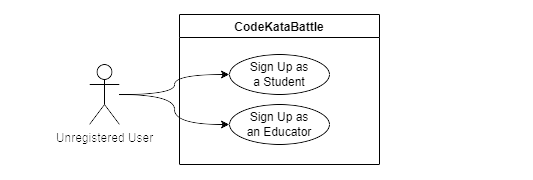
\includegraphics[width=1\linewidth]{UseCasesUU.png}
        \caption{Use Cases Diagram for Unregistered Users.} 
        \label{fig:UnregisteredUC}%
    \end{center}
\end{figure}

\begin{figure}[H]
    \begin{center}
        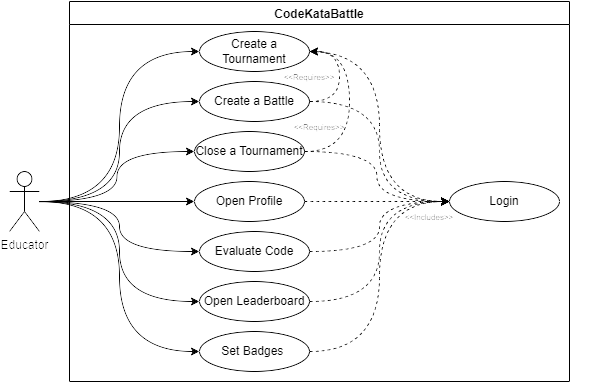
\includegraphics[width=1\linewidth]{UseCasesED.png}
        \caption{Use Cases Diagram for Educators.}
        \label{fig:EducatorUC}%
    \end{center}
\end{figure}

\begin{figure}[H]
    \begin{center}
        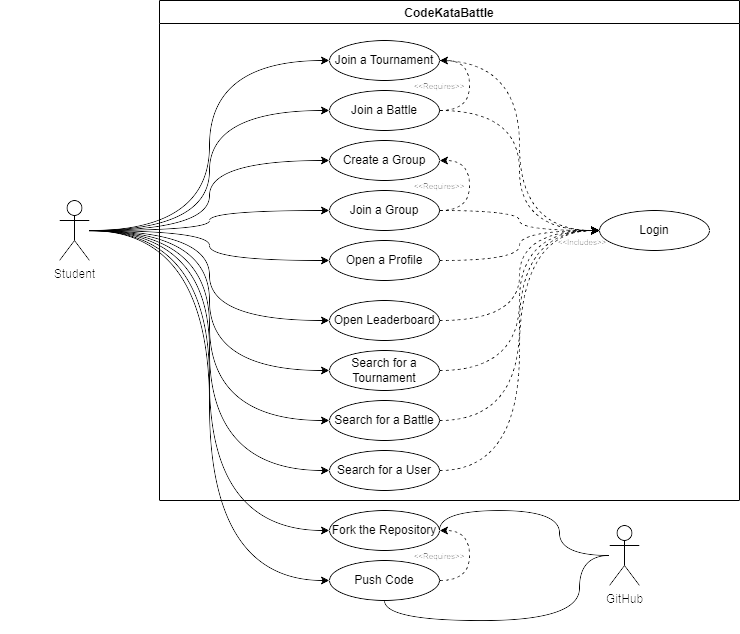
\includegraphics[width=1\linewidth]{UseCasesST.png}
        \caption{Use Cases Diagram for Students.}
        \label{fig:StudentUC}%
    \end{center}
\end{figure}

\newpage
\subsection{Use cases}
\label{subsec: use_cases}%
\newcounter{uc}
\setcounter{uc}{1}
\newcommand{\cuc}{\theuc\stepcounter{uc}}
In this section, they are explained and represented the main identified use cases.\\
There is a table with entry conditions, event flow, exit conditions and exception for each of them, and a sequence diagram that shows the messages exchanged between the entities and the called functions. \\


\subsubsection*{UC\cuc . Signup as ED}
\begin{center}
    \begin{longtable}{|l|p{0.75\linewidth}|}
        \hline
        \textbf{Actor}            & ED, eMail provider\\
        \hline
        \textbf{Entry conditions} & The ED is not already registered in CKB and has to search the CKB URL in the browser search bar \\
        \hline
        \textbf{Event Flow}       & 1 - CKB shows the login form.  \\
        & 2 - The ED clicks on “Create an Account” button.   \\
        & 3 - CKB shows the signup form.    \\
        & 4 - The ED inserts his name, surname, nickname, eMail and password in the form and also ticks on the “Signup as Educator” checkbox.  \\
        & 5 - The ED clicks on the “Register” button.  \\
        & 6 - CKB checks all the credentials.  \\
        & 7 - If credentials are correct CKB sends a confirmation eMail to the ED through the eMail provider.  \\
        & 8 - The ED clicks on the confirmation link.    \\
        \hline
        \textbf{Exit condition}   & CKB allows the ED to access to the CKB system. \\       
        \hline
        \textbf{Exceptions}       & \begin{itemize}
            \item The eMail address is already linked to an account. In this case an error message is shown and the ED is redirected to the profile creation settings.
            \item Invalid password if it is shorter than 8 characters, if it doesn’t have at least 1 number and/or 1 capital letter and/or a special character. In this case an error message is shown and the ED is redirected to the profile creation settings.
            \item  The nickname is already used. An error is shown and the ED is redirected to the profile creation settings.
        \end{itemize}\\
        \hline
        \caption{Signup as ED use case.}
        \label{tab: signup_as_ED_use_case}
    \end{longtable}
\end{center}

\begin{figure}[H]
    \begin{center}
        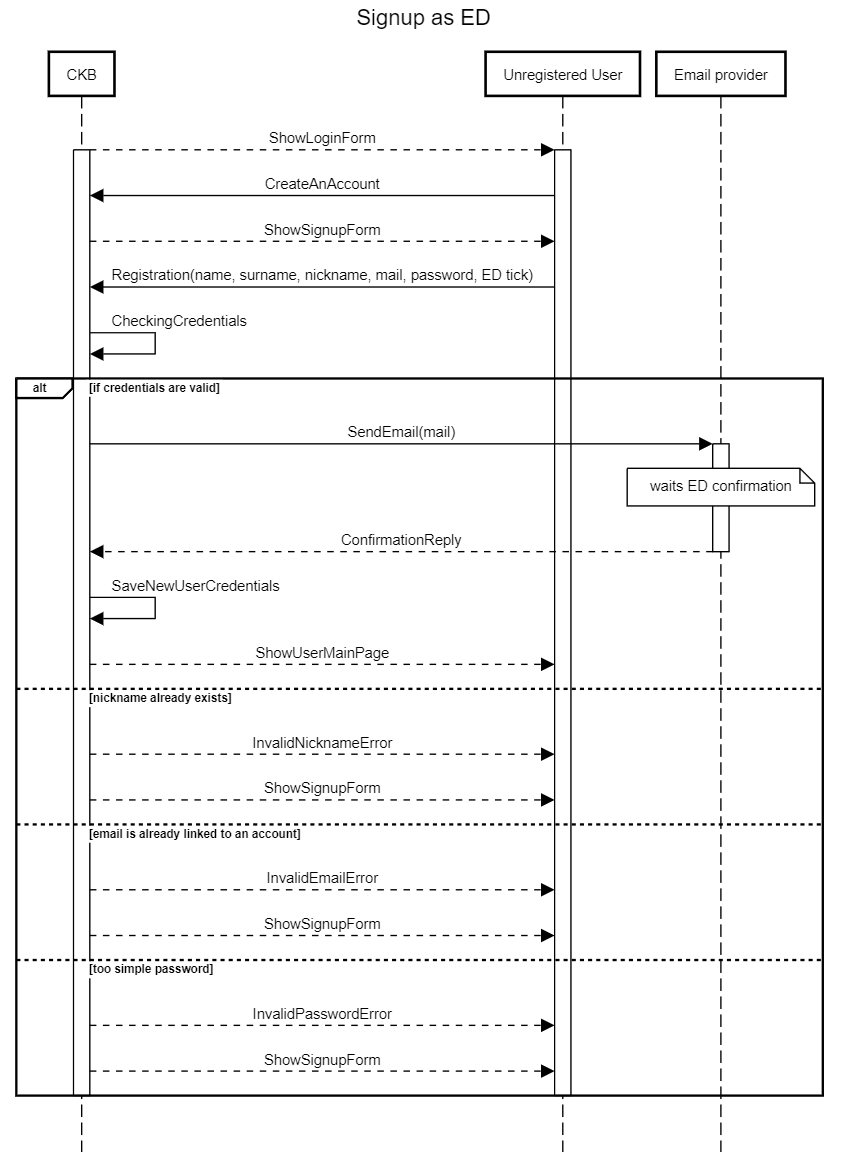
\includegraphics[width=1\linewidth]{SequenceDiagrams/Signup as ED.png}
        \caption{Signup as ED sequence diagram.}
        \label{fig:signup_as_ED_seqd}%
    \end{center}
\end{figure}

\newpage

\subsection{Requirement mapping}
\label{subsec:requirement_mapping}%
\textbf{G1 - Allow an ED to create a Tournament.}
\begin{itemize}
    \item R1: CKB allows unregistered Users to sign up.
    \item R2: CKB allows registered EDs to login.
    \item R4: CKB allows EDs to create Tournaments.
    \item R5: CKB allows EDs to grant the permissions of a Tournament to other EDs.
    \item R15: CKB allows EDs to choose which Badges to award in a certain Tournament.
    \item R17: CKB allows EDs to close a Tournament.
    \item R27: CKB sends notifications to every ST when a new Tournament is created.
    \item R50: CKB sends notifications to the ED when he receives the permission to create Battles in a Tournament.
\end{itemize}

\vspace{1.5cm}
\textbf{G2 - Allow a ST to subscribe to a specific Tournament before the registration deadline.}
\begin{itemize}
    \item R1: CKB allows unregistered Users to sign up.
    \item R3: CKB allows registered STs to login.
    \item R20: CKB allows STs to join a Tournament.
    \item R39: CKB allows STs to check the list of ongoing Tournaments.
    \item R43: CKB sends notification to every ST involved in a Tournament when the Tournament is closed and the final ranks are available.
    \item R46: CKB shall communicate with the mailing system in order to allow Users to register their account.
\end{itemize}


\vspace{1.5cm}
\textbf{G3 - Allow an ED to create a Battle.}
\begin{itemize}
    \item R6: CKB allows EDs to create Battles.
    \item R7: CKB allows EDs to uploads the code kata of a Battle.
    \item R8: CKB allows EDs to set the minimum and the maximum number of STs per group of a Battle.
    \item R9: CKB allows EDs to set a registration deadline of a Battle.
    \item R10: CKB allows EDs to set a submission deadline of a Battle.
    \item R11: CKB allows EDs to set additional configuration for the scoring system of a Battle.
    \item R12: CKB allows EDs to set functional aspects for the scoring system of a Battle.
    \item R16: CKB allows EDs to assign a score manually during the consolidation stage.
    \item R28: CKB sends notifications when a new Battle is created to every ST which is participating in the Tournament that the Battle is part of.
    \item R30: CKB creates a GH repository of the code kata when the registration deadline for the Battle expires.
    \item R31: CKB sends the link of the GH repository to every STG that participates in the Battle.
    \item R32: CKB evaluates the STG's work every time a push is made on GH and calculates Battle score for the STG.
    \item R33: CKB updates the Battle Leaderboard once a new score is registered.
    \item R46: CKB shall communicate with the mailing system in order to allow Users to register their account.
\end{itemize}


\vspace{1.5cm}
\textbf{G4 - Allow any User to visualize the profile of other Users and their Badges.}
\begin{itemize}
    \item R18: CKB allows EDs to visualize the profile of another User.
    \item R19: CKB allows STs to visualize the profile of another User.
    \item R25: CKB stores the information about the Users.
    \item R26: CKB shall ensure security of data. 
\end{itemize}


\vspace{1.5cm}
\textbf{G5 - Allow a ST to subscribe to a specific Battle before the registration deadline.}
\begin{itemize}
    \item R21: CKB allows STs to join a Battle.
    \item R22: CKB allows STs to create a new STG.
    \item R23: CKB allows STs to join a STG.
    \item R24: CKB allows STs to invite other STs in their STG.
    \item R29: CKB sends notifications to a ST when he receives an invitation to be part of STG.
    \item R31: CKB sends the link of the GH repository to every STG that participates in the Battle.
\end{itemize}


\vspace{1.5cm}
\textbf{G6 - Allow STs to submit their code before the submission deadline.}
\begin{itemize}
    \item R16: CKB allows EDs to assign a score manually during the consolidation stage.
    \item R32: CKB evaluates the STG's work every time a push is made on GH and calculates Battle score for the STG.
    \item R33: CKB updates the Battle Leaderboard once a new score is registered.
    \item R34: CKB updates the Tournament Leaderboard once a new score is registered.
    \item R37: CKB allows EDs to analyze the code of a STG.
    \item R38: CKB sends notification to every ST involved in a Tournament when the Tournament is closed and the final ranks are available.
    \item R44: CKB shall communicate with the GH API in order to calculate a new score every time a push action is made by a STG.
    \item R45: CKB shall communicate with the external tool in order to calculate the score of a STG.
    \item R47: STs need to fork the GH repository of the Battle they are participating in.
    \item R48: STs need to push their code in the GH repository in order to have their code evaluated.
\end{itemize}


\vspace{1.5cm}
\textbf{G7 - Allow an ED to set Badges for deserving STs.}
\begin{itemize}
    \item R13: CKB allows EDs to create new Badges.
    \item R14: CKB allows EDs to choose the rules related to the awarding of Badges.
    \item R15: CKB allows EDs to choose which Badges to award in a certain Tournament.
    \item R49: CKB shall assign the Badges to all STs that fulfill their requirements.
\end{itemize}


\vspace{1.5cm}
\textbf{G8 - Allow any User to view the result and the progress of a Tournament.}
\begin{itemize}
    \item R34: CKB updates the Tournament Leaderboard once a new score is registered.
    \item R40: CKB allows EDs to check the list of ongoing Tournaments.
    \item R41: CKB allows STs to check the Leaderboard of a Tournaments.
    \item R42: CKB allows EDs to check the Leaderboard of a Tournaments.
    \item R43: CKB sends notification to every ST involved in a Tournament when the Tournament is closed and the final ranks are available.
\end{itemize}


\vspace{1.5cm}
\textbf{G9 - Allow any User to view the results of a Battle.}
\begin{itemize}
    \item R33: CKB updates the Battle Leaderboard once a new score is registered.
    \item R35: CKB allows STs to check the Leaderboard of a Battle.
    \item R36: CKB allows EDs to check the Leaderboard of a Battle.
\end{itemize}

\vspace{1.5cm}
\newcounter{rtt}
\setcounter{rtt}{1}
\newcommand{\crt} {\thertt\stepcounter{rtt}}
\begin{center}
     \begin{longtable}{|l|c|c|c|c|c|c|c|c|c|}
    \hline
    \textbf{Requirements} & \textbf{G1} & \textbf{G2} & \textbf{G3} & \textbf{G4} & \textbf{G5} & \textbf{G6} & \textbf{G7} & \textbf{G8} & \textbf{G9}\\ \hline
    R\crt & \checkmark & \checkmark &  &  &  &  &  &  &  \\ \hline
    R\crt & \checkmark &  &  &  &  &  &  &  &  \\ \hline
    R\crt &  & \checkmark &  &  &  &  &  &  &  \\ \hline
    R\crt & \checkmark &  &  &  &  &  &  &  &  \\ \hline
    R\crt & \checkmark &  &  &  &  &  &  &  &  \\ \hline
    R\crt &  &  & \checkmark &  &  &  &  &  &  \\ \hline
    R\crt &  &  & \checkmark &  &  &  &  &  &  \\ \hline
    R\crt &  &  & \checkmark &  &  &  &  &  &  \\ \hline
    R\crt &  &  & \checkmark &  &  &  &  &  &  \\ \hline
    R\crt &  &  & \checkmark &  &  &  &  &  &  \\ \hline
    R\crt &  &  & \checkmark &  &  &  &  &  &  \\ \hline
    R\crt &  &  & \checkmark &  &  &  &  &  &  \\ \hline
    R\crt &  &  &  &  &  &  & \checkmark &  &  \\ \hline
    R\crt &  &  &  &  &  &  & \checkmark &  &  \\ \hline
    R\crt &\checkmark  &  &  &  &  &  & \checkmark &  &  \\ \hline
    R\crt &  &  & \checkmark &  &  & \checkmark &  &  &  \\ \hline
    R\crt &\checkmark  &  &  &  &  &  &  &  &  \\ \hline
    R\crt &  &  &  & \checkmark &  &  &  &  &  \\ \hline
    R\crt &  &  &  & \checkmark &  &  &  &  &  \\ \hline
    R\crt &  & \checkmark &  &  &  &  &  &  &  \\ \hline
    R\crt &  &  &  &  & \checkmark &  &  &  &  \\ \hline
    R\crt &  &  &  &  & \checkmark &  &  &  &  \\ \hline
    R\crt &  &  &  &  & \checkmark &  &  &  &  \\ \hline
    R\crt &  &  &  &  & \checkmark &  &  &  &  \\ \hline
    R\crt &  &  &  & \checkmark &  &  &  &  &  \\ \hline
    R\crt &  &  &  & \checkmark &  &  &  &  &  \\ \hline
    R\crt & \checkmark &  &  &  &  &  &  &  &  \\ \hline
    R\crt &  &  & \checkmark &  &  &  &  &  &  \\ \hline
    R\crt &  &  &  &  & \checkmark &  &  &  &  \\ \hline
    R\crt &  &  & \checkmark &  &  &  &  &  &  \\ \hline
    R\crt &  &  & \checkmark &  & \checkmark &  &  &  &  \\ \hline
    R\crt &  &  & \checkmark &  &  & \checkmark &  &  &  \\ \hline
    R\crt &  &  & \checkmark &  &  & \checkmark &  &  & \checkmark \\ \hline
    R\crt &  &  &  &  &  & \checkmark &  & \checkmark &  \\ \hline
    R\crt &  &  &  &  &  &  &  &  & \checkmark \\ \hline
    R\crt &  &  &  &  &  &  &  &  & \checkmark \\ \hline
    R\crt &  &  &  &  &  & \checkmark &  &  &  \\ \hline
    R\crt &  &  &  &  &  & \checkmark &  &  &  \\ \hline
    R\crt &  & \checkmark &  &  &  &  &  &  &  \\ \hline
    R\crt &  &  &  &  &  &  &  & \checkmark &  \\ \hline
    R\crt &  &  &  &  &  &  &  & \checkmark &  \\ \hline
    R\crt &  &  &  &  &  &  &  & \checkmark &  \\ \hline
    R\crt &  &  \checkmark&  &  &  &  &  & \checkmark &  \\ \hline
    R\crt &  &  &  &  &  & \checkmark &  &  &  \\ \hline
    R\crt &  &  &  &  &  & \checkmark &  &  &  \\ \hline
    R\crt &  &  \checkmark& \checkmark &  &  &  &  &  &  \\ \hline
    R\crt &  &  &  &  &  & \checkmark &  &  &  \\ \hline
    R\crt &  &  &  &  &  & \checkmark &  &  &  \\ \hline
    R\crt &  &  &  &  &  &  & \checkmark &  &  \\ \hline
    R\crt & \checkmark &  &  &  &  &  &  &  &   \\ \hline
\caption{Traceability Matrix for Goals and Requirements}
\label{tab:traceability}
\end{longtable}
\end{center}


\section{Performance requirements}
\label{sec:performance_requirements}%
---

\newpage
\section{Design constraints}
\label{sec:design_constraints}%

\subsection{Standard compliance}
\label{subsec:standard compliance}%%
---

\subsection{Hardware limitations}
\label{subsec:hardware_limitations}%
---

\subsection{Any other constraint}
\label{subsec:any_other_constraint}%
---

\section{Software system attributes}
\label{sec:software_system_attributes}%

\subsection{Reliability}
\label{subsec:reliability}%
---

\subsection{Availability}
\label{subsec:availability}%
---

\subsection{Security}
\label{subsec:security}%
---

\subsection{Maintainability}
\label{subsec:maintainability}%
---

\subsection{Portability}
\label{subsec:portability}%
---